\lecture{9}{10.17}
\begin{eg}
    $X\sim U[-1,1]$ ,对应的密度函数:
    \begin{align*}
        f_X\left( x \right) = \begin{cases}
            0,&x< -1 \text{ or } x>1\\
            \frac{1}{2},&x\in [-1,1]
        \end{cases}
    .\end{align*}

    同理$Y\sim U[-1,1]$,求$Z=\left| X-Y \right| $ 的分布函数
\end{eg}
解:$Z$ 的取值:[0,2]

\begin{align*}
    F_Z\left( z \right) &=P\left\{ Z\le z \right\} \\
    &= P\left\{ \left| X-Y \right| \le z \right\} \\
    &= \begin{cases}
        0,&z<0\\
        1,&z\ge 2\\
     P\left\{ -z\le X-Y\le z \right\} ,&z\in [0,2)
    \end{cases}
.\end{align*}

其中\[
    P\left\{ z-z\le X-Y\le z \right\} =\iint_{-z\le x-y\le z} f\left( x,y \right) \mathrm{d}x \mathrm{d}y
.\] 

通过$f_X\text{和}f_Y$ 求联合密度函数:$X,Y$ 独立,即$f\left( x,y \right) =f_X\left( x \right) f_Y\left( y \right) $
\begin{align*}
    f\left( x,y \right) =\begin{cases}
        0,&x,y< -1 \text{ or } x,y>1\\
        \frac{1}{4},&x,y \in [-1,1]
    \end{cases}
.\end{align*}
\begin{align*}
    P\left\{ -z\le X-Y\le z \right\} =\underset{-z\le x-y\le z,x,y\in [-1,1]}{\iint} \frac{1}{4} \mathrm{d}x\mathrm{d}y
.\end{align*}

画图确认积分区域:
\begin{figure}[htbp]
    \centering
    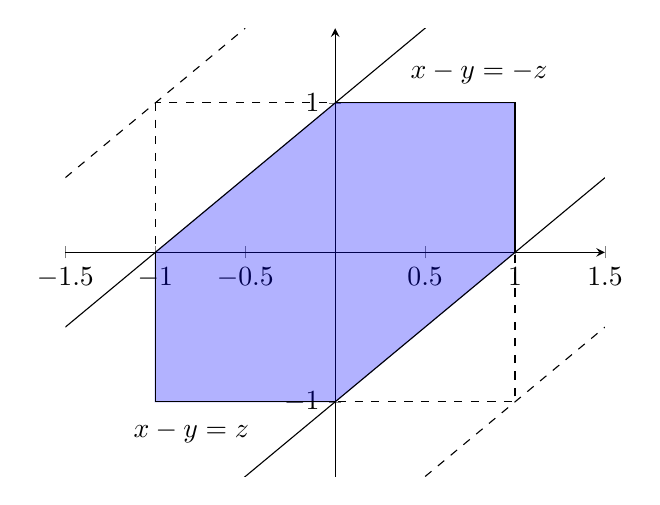
\begin{tikzpicture}
        \begin{axis}[
            xmin=-1.5, xmax=1.5,
            ymin=-1.5, ymax=1.5,
            axis lines=middle,
        ]
            \filldraw [color=blue, opacity=0.3] (-1,0)--(0,1)--(1,1)--(1,0)--(0,-1)--(-1,-1)--(-1,0);
            \draw [dashed] (-1.5,0.5)--(-0.5,1.5);
            \draw [dashed] (0.5,-1.5)--(1.5,-0.5);
            \addplot[domain=-1.5:1.5]{x-1};
            \addplot[domain=-1.5:1.5]{x+1};
            \draw [dashed] (-1,1) rectangle (1,-1) node at(0,0) {$ $};
            \draw [] (0,1)--(1,1)--(1,0);
            \draw [] (0,-1)--(-1,-1)--(-1,0);
            \node at(-0.8,-1.2) {$x-y=z$};
            \node at(0.8,1.2) {$x-y=-z$};
        \end{axis}
    \end{tikzpicture}
\end{figure}
\begin{notation}
    i.i.d. : 独立同分布
\end{notation}
\begin{notation}
    伽马分布$\varGamma\left( \alpha,\beta \right) $ 的密度函数:
    \begin{align*}
        f\left( x \right) =\begin{cases}
            \displaystyle{\frac{\beta^{\alpha}}{\Gamma\left( \alpha \right) }}x^{\alpha-1}\mathrm{e}^{-\beta x}, &x\ge 0\\
            0,&x<0
        \end{cases}
    .\end{align*}
\end{notation}
\begin{notation}
    重点题目:3.6.2
\end{notation}
\section{数字特征}%
\label{sec:数字特征}
\[
    \text{数字特征}\begin{cases}
        \text{数学期望:}E\left( X \right) \\
        \text{方差:}D\left( X \right) \text{ or }\mathrm{Var}\left( X \right) \\
        \text{协方差:}\mathrm{cov}\left( X,Y \right) \\
        \text{相关系数:}\rho\left( X,Y \right) \\
        \text{矩:}E\left( X \right) ^{k} \text{ and } E\left( X-EX \right) ^{k}
    \end{cases}
.\] 
\begin{notation}
    $D\left( X \right) =E\left( X-EX \right) ^2$ 

    $\text{cov}\left( X,Y \right) =E\left( \left( X-EX \right) \left( Y-EY \right)  \right) $

    $ \rho\left( X,Y \right) =\displaystyle{\frac{\text{cov}\left( X,Y \right) }{\sqrt{DX} \sqrt{DY} }}$
\end{notation}
\begin{notation}
    $|\rho_{X,Y}|\in [0,1]$ 
    
    $\rho$ 越大越线性相关,$\rho>0.8$ 时基本可以确定为线性相关
\end{notation}
\begin{notation}
    矩(moment)是最一般的概念

    矩分为两大类:$k$ 阶原点矩和$k$ 阶中心矩

    原点矩:$E\left( X \right) ^{k}$

    中心矩:$E\left( X-EX \right) ^{k}$

    $k+l$ 阶混合中心矩:$E\left( \left( X-EX \right) ^{k}\left( Y-EY \right) ^{l} \right) $
\end{notation}
\begin{eg}
    数学期望为一阶原点矩

    方差为一阶中心矩

    协方差为二阶混合中心矩
\end{eg}
\begin{notation}
    可以写出无穷阶的中心矩等同于通过泰勒原理得出分布函数
    
    本章重点:如何计算任意随机变量有关函数的数学期望

    唯一计算公式:4.1.5和4.1.6
\end{notation}
\subsection{数学期望}%
\label{sub:数学期望}
\begin{defi}
    离散型随机变量$X$ 的分布律:$P\left\{ X=x_i \right\} =p_i,i=1,2,\ldots$ 

    若级数$\displaystyle{\sum_{i=1}^{+\infty} x_ip_i}$ \textbf{绝对收敛}($\displaystyle{\sum_{i=1}^{+\infty} \left| x_i \right| p_i<+\infty}$),则$X$ 的数学期望\textbf{存在}($x_i$ 为取值,$p_i$ 为权重,$p_i\ge 0$)
    \[
        E\left( X \right) =EX=\sum_{i=1}^{+\infty} x_iP\left\{ X=x_i \right\} =\sum_{i=1}^{+\infty} x_ip_i
    .\] 
\end{defi}
\begin{rrule}
    当一个随机变量的密度函数与分布律已知:$X\to f\left( x \right),P\left\{ X=x_i \right\} =p_i $

    即可以求关于$X$ 函数的数学期望(公式4.1.5):
    \begin{align*}
        E\left( g\left( X \right)  \right) =\begin{cases}
            \displaystyle{\sum_{i=1}^{+\infty} g\left( x_i \right) P\left\{ X=x_i \right\} },&X\text{离散}\\
            \displaystyle{\int_{-\infty}^{+\infty} g\left( x \right) f\left( x \right)  \mathrm{d}x},&X\text{连续}
        \end{cases}
    .\end{align*}
\end{rrule}
\begin{rrule}
    扩展至二阶:$\left( X,Y \right) \to P\left\{ X=x_{i},Y=y_{j} \right\} ,f\left( x,y \right) $ 

    关于$\left( X,Y \right) $ 的函数的数学期望(公式4.1.6):
    \begin{align*}
        E\left( g\left( X,Y \right)  \right) =\begin{cases}
            \displaystyle{\sum_{i=1}^{+\infty}{\sum_{j=1}^{+\infty} g\left( x_{i},y_{j} \right) P\left\{ X=x_{i},Y=y_{j} \right\}} },&\text{离散}\\
            \displaystyle{\int_{-\infty}^{+\infty}{\int_{-\infty}^{+\infty} g\left( x,y \right) f\left( x,y \right)  \mathrm{d}x} \mathrm{d}y},&\text{连续}
        \end{cases}
    .\end{align*}
\end{rrule}
\begin{notation}
    柯西分布:\[
        f\left( x \right) =\frac{1}{\pi\left( 1+x^2 \right) },x\in \mathbb{R}
    .\] 
\end{notation}
常见分布数学期望:
\begin{notation}
    伯努利分布$X\sim B\left( n,p \right) $ :$EX=np$ 

    泊松分布$X\sim P\left( \lambda \right) \left( \lambda>0 \right) $ :$EX=\lambda$ 

    柯西分布:$EX$ 不存在(柯西分布不绝对收敛)
\end{notation}
\begin{notation}
    柯西活了68岁,21岁成名(导师拉格朗日),27岁当选法国科学院院士
\end{notation}



